\section{Введение}
\label{sec:intro}

На 3 курсе ФПМИ МФТИ проводится курс по распределенным системам. Также этот курс читается на 4 курсе ФКН ВШЭ и 2 курсе ШАД.

При прохождении курса студенты решают практические задачи: написание распределенных сервисов с помощью фреймворка курса whirl \cite{whirl}. Код студентов запускается внутри среды исполнения, которая является детерминированной симуляцией распределенной системы.

Таким образом, основными пользователями фреймворка являются студенты. Далее мы будем отождествлять два этих слова.

Имеется потребность в написании тестирующего инструмента для данного курса распределенных систем. На данный момент тестирование является перебором некоторого количества состояний распределенного сервиса. На некоторых видах задач требуется увеличить покрытие тестирования.

Интеграция фреймворка курса с какими-либо аналогами невозможна, так как фреймворк является самописной разработкой на С++.

\subsection{Постановка задачи}

Инструмент должен решать задачу тестирования распределенной системы, внутри которой исполняется код студента.

Распределенную систему мы представим в виде набора узлов, объединенных в общую сеть. Узлы могут коммуницировать друг с другом только с помощью отправки сообщений.

Сеть мы считаем асинхронной и недетерминированной – она может произвольно задерживать и переупорядочивать отправляемые узлами сообщения. Если система будет корректно работать в асинхронной сети, то и в реальной, частично синхронной сети тоже.

Внутри узла исполняются недетерминированные программы. Также узлы могут отказывать, то есть перезагружаться в произвольные моменты и/или навсегда отключаться.

Мы считаем, что набор узлов системы реализует некоторый распределенный сервис, с которым клиенты взаимодействуют через протокол RPC. 

Клиенты тоже являются узлами сети. 

Они посылают системе запросы и получают ответы, в результате возникает конкурентная история, состоящая из отрезков запросов (рис.~\ref{fig:history_example}). Свойства системы формулируются как утверждения про допустимые истории, которые может порождать система.

\begin{figure}[h]
    \centering
    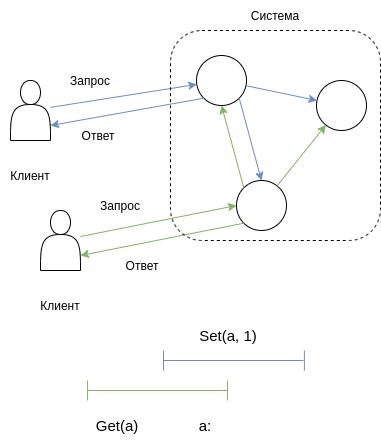
\includegraphics[width=0.5\textwidth]{img/task.png}
    \caption{Пример истории запросов}
    \label{fig:history_example}
\end{figure}

В данной работе нас прежде всего интересует задача репликации, так что распределенный сервис  представляет собой хранилище данных с операциями Set и Get, а свойство, которое мы ожидаем от системы – модель согласованности \cite{consistency}, в первую очередь – линеаризуемость \cite{linearizability}.

Наконец, сформулируем задачу – по реализации узлов системы проверить выполнение заявленных свойств независимо от поведения сети между узлами, часов и т.д.

\subsection{Цель работы}

Цель работы состоит в реализации части библиотеки Roren, отвечающей за перевод и выполнение pipeline-ов поверх YT. Компонент должен позволять запускать произвольные графы обработки данных, выражаемые операциями Map/Reduce.

Получившаяся реализация в сравнении с текущей должна:
\begin{itemize}
    \item Переводить pipeline-ы в графы с меньшим количеством YT операций
    \item Иметь расширяемый на более сложные YT операции алгоритм трансляции
\end{itemize}

\subsection{План работы}

Во второй главе мы рассмотрим дизайн библиотеки Roren: от API pipeline-ов до запуска YT операций.

В третьей главе рассмотрим реализацию компонента, производящего трансляцию. Мы изложим этапы перевода roren графа в граф YT операций, алгоритм трансляции, и детально остановимся на компоненте оптимизатора.

В четвертой главе посмотрим на примеры графов и их трансляций, обсудим тестирование.

В последней главе мы поговорим о результатах работы и обсудим пути развития компонента.

